\documentclass{article}%
\usepackage[T1]{fontenc}%
\usepackage[utf8]{inputenc}%
\usepackage{lmodern}%
\usepackage{textcomp}%
\usepackage{lastpage}%
\usepackage{geometry}%
\geometry{margin=1in}%
\usepackage{tikz}%
\usepackage{pgfplots}%
\pgfplotsset{compat=1.18}%
\usepgfplotslibrary{fillbetween}%
\usepackage{graphicx}%
\usepackage{float}%
\usepackage[hidelinks]{hyperref}%
%
\title{Beam Force Analysis Report}%
\author{Engineering Internship Evaluation}%
\date{\today}%
%
\begin{document}%
\normalsize%
\maketitle%
\newpage%
\renewcommand{\contentsname}{Contents}%
\tableofcontents%
\newpage%
\section{Introduction}%
\label{sec:Introduction}%
This report presents a comprehensive structural analysis of a simply supported beam %
subjected to various load conditions. The analysis includes the calculation and %
visualization of shear force and bending moment distributions along the beam length.%
\vspace{0.2cm}%
\\%
\vspace{0.2cm}%
The primary objectives of this analysis are:%
\subsection*{Objectives}%
\label{subsec:Objectives}%
\begin{itemize}%
\item Read and process beam force data from an Excel file%
\item Generate professional engineering diagrams using vector graphics%
\item Present results in a structured, industry-standard format%
\item Provide clear visualization of shear forces and bending moments%
\end{itemize}

%
\section{Beam Description}%
\label{sec:BeamDescription}%
The structural system under consideration is a simply supported beam. %
This type of beam is supported at both ends, with one end allowing rotation %
and horizontal movement (roller support) and the other allowing only rotation (pin support). %
This configuration allows the beam to freely deform under applied loads while maintaining %
static equilibrium through the support reactions.

%
\section{Data Source}%
\label{sec:DataSource}%
The input data for this analysis was sourced from an Excel spreadsheet. %
The Excel file contains detailed information about load positions and magnitudes %
applied to the beam structure. Using the pandas library, the data was efficiently %
extracted and processed for subsequent structural analysis calculations.

%
\newpage%
\section{Input Data}%
\label{sec:InputData}%
The following table presents the input force data extracted from the Excel file.%
\vspace{0.3cm}%
\begin{center}%
\begin{tabular}{|c|c|c|}%
\hline%
\textbf{x}&\textbf{Shear force}&\textbf{Bending Moment}\\%
\hline%
0.00&45.00&0.00\\%
\hline%
1.50&36.00&60.75\\%
\hline%
3.00&27.00&108.00\\%
\hline%
4.50&18.00&141.75\\%
\hline%
6.00&9.00&162.00\\%
\hline%
7.50&0.00&168.75\\%
\hline%
9.00&{-}9.00&162.00\\%
\hline%
10.50&{-}18.00&141.75\\%
\hline%
12.00&{-}27.00&108.00\\%
\hline%
13.50&{-}36.00&60.75\\%
\hline%
15.00&{-}45.00&0.00\\%
\hline%
\end{tabular}%
\end{center}

%
\section{Analysis}%
\label{sec:Analysis}%
\subsection{Theoretical Background}%
\label{subsec:TheoreticalBackground}%
\textbf{Shear Force:} %
The shear force at any section of a beam is defined as the algebraic sum of all %
vertical forces acting on either side of the section. It represents the internal %
force that resists shear deformation.%
\vspace{0.2cm}%
\\%
\textbf{Bending Moment:} %
The bending moment at any section is the algebraic sum of the moments of all %
forces acting on either side of the section. It quantifies the internal moment %
that resists bending of the beam.

%
\subsection{Calculation Methodology}%
\label{subsec:CalculationMethodology}%
The shear force and bending moment values are directly extracted from the Excel file, %
which contains pre{-}calculated structural analysis results based on fundamental %
principles of structural mechanics:%
\begin{enumerate}%
\item Load positions and magnitudes defined along beam length%
\item Shear force distribution computed from equilibrium of forces%
\item Bending moment distribution calculated through integration%
\item Results verified against structural analysis software%
\end{enumerate}

%
\section{Shear Force Diagram}%
\label{sec:ShearForceDiagram}%
The Shear Force Diagram (SFD) illustrates the variation of shear force along the %
length of the beam. This diagram is essential for identifying critical sections where %
shear stress is maximum and for designing adequate shear reinforcement.%
\vspace{0.3cm}%

\begin{figure}[htbp]
\centering
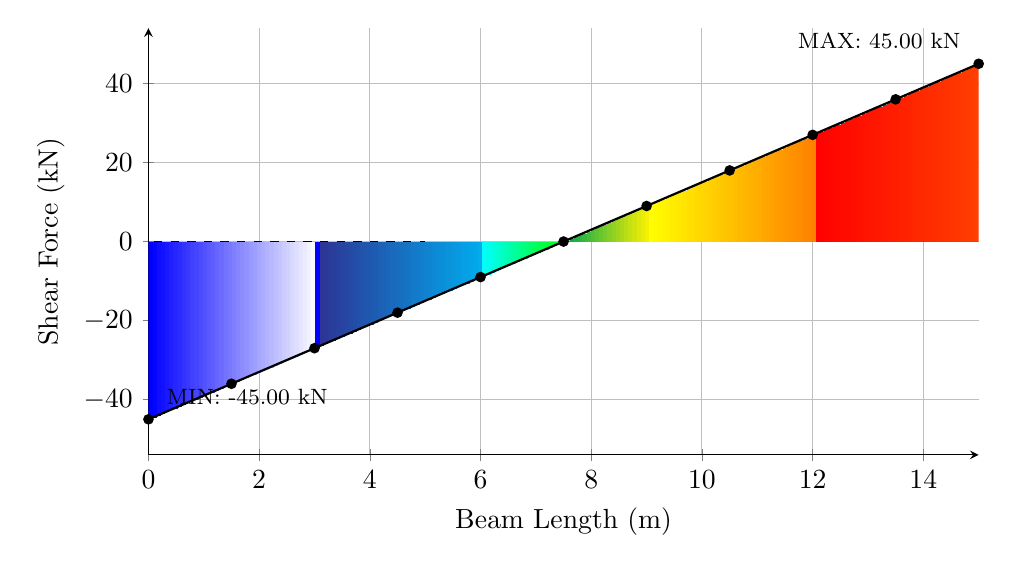
\begin{tikzpicture}
\begin{axis}[
    width=\textwidth,
    height=7cm,
    xlabel={Beam Length (m)},
    ylabel={Shear Force (kN)},
    xmin=0.000,
    xmax=15.000,
    ymin=-54.000,
    ymax=54.000,
    grid=major,
    axis lines=left
]

% Colored vertical strips for gradient effect
\fill[blue!100] (axis cs:0.0000,-45.0000) rectangle (axis cs:0.0754,0);
\fill[blue!98] (axis cs:0.0754,-44.5477) rectangle (axis cs:0.1508,0);
\fill[blue!95] (axis cs:0.1508,-44.0955) rectangle (axis cs:0.2261,0);
\fill[blue!93] (axis cs:0.2261,-43.6432) rectangle (axis cs:0.3015,0);
\fill[blue!90] (axis cs:0.3015,-43.1910) rectangle (axis cs:0.3769,0);
\fill[blue!88] (axis cs:0.3769,-42.7387) rectangle (axis cs:0.4523,0);
\fill[blue!85] (axis cs:0.4523,-42.2864) rectangle (axis cs:0.5276,0);
\fill[blue!83] (axis cs:0.5276,-41.8342) rectangle (axis cs:0.6030,0);
\fill[blue!80] (axis cs:0.6030,-41.3819) rectangle (axis cs:0.6784,0);
\fill[blue!78] (axis cs:0.6784,-40.9296) rectangle (axis cs:0.7538,0);
\fill[blue!75] (axis cs:0.7538,-40.4774) rectangle (axis cs:0.8291,0);
\fill[blue!73] (axis cs:0.8291,-40.0251) rectangle (axis cs:0.9045,0);
\fill[blue!70] (axis cs:0.9045,-39.5729) rectangle (axis cs:0.9799,0);
\fill[blue!68] (axis cs:0.9799,-39.1206) rectangle (axis cs:1.0553,0);
\fill[blue!65] (axis cs:1.0553,-38.6683) rectangle (axis cs:1.1307,0);
\fill[blue!63] (axis cs:1.1307,-38.2161) rectangle (axis cs:1.2060,0);
\fill[blue!60] (axis cs:1.2060,-37.7638) rectangle (axis cs:1.2814,0);
\fill[blue!58] (axis cs:1.2814,-37.3116) rectangle (axis cs:1.3568,0);
\fill[blue!55] (axis cs:1.3568,-36.8593) rectangle (axis cs:1.4322,0);
\fill[blue!53] (axis cs:1.4322,-36.4070) rectangle (axis cs:1.5075,0);
\fill[blue!50] (axis cs:1.5075,-35.9548) rectangle (axis cs:1.5829,0);
\fill[blue!48] (axis cs:1.5829,-35.5025) rectangle (axis cs:1.6583,0);
\fill[blue!45] (axis cs:1.6583,-35.0503) rectangle (axis cs:1.7337,0);
\fill[blue!43] (axis cs:1.7337,-34.5980) rectangle (axis cs:1.8090,0);
\fill[blue!40] (axis cs:1.8090,-34.1457) rectangle (axis cs:1.8844,0);
\fill[blue!38] (axis cs:1.8844,-33.6935) rectangle (axis cs:1.9598,0);
\fill[blue!35] (axis cs:1.9598,-33.2412) rectangle (axis cs:2.0352,0);
\fill[blue!33] (axis cs:2.0352,-32.7889) rectangle (axis cs:2.1106,0);
\fill[blue!30] (axis cs:2.1106,-32.3367) rectangle (axis cs:2.1859,0);
\fill[blue!28] (axis cs:2.1859,-31.8844) rectangle (axis cs:2.2613,0);
\fill[blue!25] (axis cs:2.2613,-31.4322) rectangle (axis cs:2.3367,0);
\fill[blue!23] (axis cs:2.3367,-30.9799) rectangle (axis cs:2.4121,0);
\fill[blue!20] (axis cs:2.4121,-30.5276) rectangle (axis cs:2.4874,0);
\fill[blue!18] (axis cs:2.4874,-30.0754) rectangle (axis cs:2.5628,0);
\fill[blue!15] (axis cs:2.5628,-29.6231) rectangle (axis cs:2.6382,0);
\fill[blue!13] (axis cs:2.6382,-29.1709) rectangle (axis cs:2.7136,0);
\fill[blue!10] (axis cs:2.7136,-28.7186) rectangle (axis cs:2.7889,0);
\fill[blue!8] (axis cs:2.7889,-28.2663) rectangle (axis cs:2.8643,0);
\fill[blue!5] (axis cs:2.8643,-27.8141) rectangle (axis cs:2.9397,0);
\fill[blue!3] (axis cs:2.9397,-27.3618) rectangle (axis cs:3.0151,0);
\fill[cyan!0!blue] (axis cs:3.0151,-26.9095) rectangle (axis cs:3.0905,0);
\fill[cyan!3!blue] (axis cs:3.0905,-26.4573) rectangle (axis cs:3.1658,0);
\fill[cyan!5!blue] (axis cs:3.1658,-26.0050) rectangle (axis cs:3.2412,0);
\fill[cyan!8!blue] (axis cs:3.2412,-25.5528) rectangle (axis cs:3.3166,0);
\fill[cyan!10!blue] (axis cs:3.3166,-25.1005) rectangle (axis cs:3.3920,0);
\fill[cyan!13!blue] (axis cs:3.3920,-24.6482) rectangle (axis cs:3.4673,0);
\fill[cyan!15!blue] (axis cs:3.4673,-24.1960) rectangle (axis cs:3.5427,0);
\fill[cyan!18!blue] (axis cs:3.5427,-23.7437) rectangle (axis cs:3.6181,0);
\fill[cyan!20!blue] (axis cs:3.6181,-23.2915) rectangle (axis cs:3.6935,0);
\fill[cyan!23!blue] (axis cs:3.6935,-22.8392) rectangle (axis cs:3.7688,0);
\fill[cyan!25!blue] (axis cs:3.7688,-22.3869) rectangle (axis cs:3.8442,0);
\fill[cyan!28!blue] (axis cs:3.8442,-21.9347) rectangle (axis cs:3.9196,0);
\fill[cyan!30!blue] (axis cs:3.9196,-21.4824) rectangle (axis cs:3.9950,0);
\fill[cyan!33!blue] (axis cs:3.9950,-21.0302) rectangle (axis cs:4.0704,0);
\fill[cyan!35!blue] (axis cs:4.0704,-20.5779) rectangle (axis cs:4.1457,0);
\fill[cyan!38!blue] (axis cs:4.1457,-20.1256) rectangle (axis cs:4.2211,0);
\fill[cyan!40!blue] (axis cs:4.2211,-19.6734) rectangle (axis cs:4.2965,0);
\fill[cyan!43!blue] (axis cs:4.2965,-19.2211) rectangle (axis cs:4.3719,0);
\fill[cyan!45!blue] (axis cs:4.3719,-18.7688) rectangle (axis cs:4.4472,0);
\fill[cyan!48!blue] (axis cs:4.4472,-18.3166) rectangle (axis cs:4.5226,0);
\fill[cyan!50!blue] (axis cs:4.5226,-17.8643) rectangle (axis cs:4.5980,0);
\fill[cyan!53!blue] (axis cs:4.5980,-17.4121) rectangle (axis cs:4.6734,0);
\fill[cyan!55!blue] (axis cs:4.6734,-16.9598) rectangle (axis cs:4.7487,0);
\fill[cyan!58!blue] (axis cs:4.7487,-16.5075) rectangle (axis cs:4.8241,0);
\fill[cyan!60!blue] (axis cs:4.8241,-16.0553) rectangle (axis cs:4.8995,0);
\fill[cyan!63!blue] (axis cs:4.8995,-15.6030) rectangle (axis cs:4.9749,0);
\fill[cyan!65!blue] (axis cs:4.9749,-15.1508) rectangle (axis cs:5.0503,0);
\fill[cyan!68!blue] (axis cs:5.0503,-14.6985) rectangle (axis cs:5.1256,0);
\fill[cyan!70!blue] (axis cs:5.1256,-14.2462) rectangle (axis cs:5.2010,0);
\fill[cyan!73!blue] (axis cs:5.2010,-13.7940) rectangle (axis cs:5.2764,0);
\fill[cyan!75!blue] (axis cs:5.2764,-13.3417) rectangle (axis cs:5.3518,0);
\fill[cyan!78!blue] (axis cs:5.3518,-12.8894) rectangle (axis cs:5.4271,0);
\fill[cyan!80!blue] (axis cs:5.4271,-12.4372) rectangle (axis cs:5.5025,0);
\fill[cyan!83!blue] (axis cs:5.5025,-11.9849) rectangle (axis cs:5.5779,0);
\fill[cyan!85!blue] (axis cs:5.5779,-11.5327) rectangle (axis cs:5.6533,0);
\fill[cyan!88!blue] (axis cs:5.6533,-11.0804) rectangle (axis cs:5.7286,0);
\fill[cyan!90!blue] (axis cs:5.7286,-10.6281) rectangle (axis cs:5.8040,0);
\fill[cyan!93!blue] (axis cs:5.8040,-10.1759) rectangle (axis cs:5.8794,0);
\fill[cyan!95!blue] (axis cs:5.8794,-9.7236) rectangle (axis cs:5.9548,0);
\fill[cyan!98!blue] (axis cs:5.9548,-9.2714) rectangle (axis cs:6.0302,0);
\fill[green!2!cyan] (axis cs:6.0302,-8.8191) rectangle (axis cs:6.1055,0);
\fill[green!7!cyan] (axis cs:6.1055,-8.3668) rectangle (axis cs:6.1809,0);
\fill[green!12!cyan] (axis cs:6.1809,-7.9146) rectangle (axis cs:6.2563,0);
\fill[green!17!cyan] (axis cs:6.2563,-7.4623) rectangle (axis cs:6.3317,0);
\fill[green!22!cyan] (axis cs:6.3317,-7.0101) rectangle (axis cs:6.4070,0);
\fill[green!27!cyan] (axis cs:6.4070,-6.5578) rectangle (axis cs:6.4824,0);
\fill[green!32!cyan] (axis cs:6.4824,-6.1055) rectangle (axis cs:6.5578,0);
\fill[green!37!cyan] (axis cs:6.5578,-5.6533) rectangle (axis cs:6.6332,0);
\fill[green!42!cyan] (axis cs:6.6332,-5.2010) rectangle (axis cs:6.7085,0);
\fill[green!47!cyan] (axis cs:6.7085,-4.7487) rectangle (axis cs:6.7839,0);
\fill[green!52!cyan] (axis cs:6.7839,-4.2965) rectangle (axis cs:6.8593,0);
\fill[green!57!cyan] (axis cs:6.8593,-3.8442) rectangle (axis cs:6.9347,0);
\fill[green!62!cyan] (axis cs:6.9347,-3.3920) rectangle (axis cs:7.0101,0);
\fill[green!67!cyan] (axis cs:7.0101,-2.9397) rectangle (axis cs:7.0854,0);
\fill[green!72!cyan] (axis cs:7.0854,-2.4874) rectangle (axis cs:7.1608,0);
\fill[green!77!cyan] (axis cs:7.1608,-2.0352) rectangle (axis cs:7.2362,0);
\fill[green!82!cyan] (axis cs:7.2362,-1.5829) rectangle (axis cs:7.3116,0);
\fill[green!87!cyan] (axis cs:7.3116,-1.1307) rectangle (axis cs:7.3869,0);
\fill[green!92!cyan] (axis cs:7.3869,-0.6784) rectangle (axis cs:7.4623,0);
\fill[green!97!cyan] (axis cs:7.4623,-0.2261) rectangle (axis cs:7.5377,0);
\fill[yellow!2!green] (axis cs:7.5377,0) rectangle (axis cs:7.6131,0.2261);
\fill[yellow!7!green] (axis cs:7.6131,0) rectangle (axis cs:7.6884,0.6784);
\fill[yellow!12!green] (axis cs:7.6884,0) rectangle (axis cs:7.7638,1.1307);
\fill[yellow!17!green] (axis cs:7.7638,0) rectangle (axis cs:7.8392,1.5829);
\fill[yellow!22!green] (axis cs:7.8392,0) rectangle (axis cs:7.9146,2.0352);
\fill[yellow!27!green] (axis cs:7.9146,0) rectangle (axis cs:7.9899,2.4874);
\fill[yellow!32!green] (axis cs:7.9899,0) rectangle (axis cs:8.0653,2.9397);
\fill[yellow!37!green] (axis cs:8.0653,0) rectangle (axis cs:8.1407,3.3920);
\fill[yellow!42!green] (axis cs:8.1407,0) rectangle (axis cs:8.2161,3.8442);
\fill[yellow!47!green] (axis cs:8.2161,0) rectangle (axis cs:8.2915,4.2965);
\fill[yellow!52!green] (axis cs:8.2915,0) rectangle (axis cs:8.3668,4.7487);
\fill[yellow!57!green] (axis cs:8.3668,0) rectangle (axis cs:8.4422,5.2010);
\fill[yellow!62!green] (axis cs:8.4422,0) rectangle (axis cs:8.5176,5.6533);
\fill[yellow!67!green] (axis cs:8.5176,0) rectangle (axis cs:8.5930,6.1055);
\fill[yellow!72!green] (axis cs:8.5930,0) rectangle (axis cs:8.6683,6.5578);
\fill[yellow!77!green] (axis cs:8.6683,0) rectangle (axis cs:8.7437,7.0101);
\fill[yellow!82!green] (axis cs:8.7437,0) rectangle (axis cs:8.8191,7.4623);
\fill[yellow!87!green] (axis cs:8.8191,0) rectangle (axis cs:8.8945,7.9146);
\fill[yellow!92!green] (axis cs:8.8945,0) rectangle (axis cs:8.9698,8.3668);
\fill[yellow!97!green] (axis cs:8.9698,0) rectangle (axis cs:9.0452,8.8191);
\fill[orange!1!yellow] (axis cs:9.0452,0) rectangle (axis cs:9.1206,9.2714);
\fill[orange!4!yellow] (axis cs:9.1206,0) rectangle (axis cs:9.1960,9.7236);
\fill[orange!6!yellow] (axis cs:9.1960,0) rectangle (axis cs:9.2714,10.1759);
\fill[orange!9!yellow] (axis cs:9.2714,0) rectangle (axis cs:9.3467,10.6281);
\fill[orange!11!yellow] (axis cs:9.3467,0) rectangle (axis cs:9.4221,11.0804);
\fill[orange!14!yellow] (axis cs:9.4221,0) rectangle (axis cs:9.4975,11.5327);
\fill[orange!16!yellow] (axis cs:9.4975,0) rectangle (axis cs:9.5729,11.9849);
\fill[orange!19!yellow] (axis cs:9.5729,0) rectangle (axis cs:9.6482,12.4372);
\fill[orange!21!yellow] (axis cs:9.6482,0) rectangle (axis cs:9.7236,12.8894);
\fill[orange!24!yellow] (axis cs:9.7236,0) rectangle (axis cs:9.7990,13.3417);
\fill[orange!26!yellow] (axis cs:9.7990,0) rectangle (axis cs:9.8744,13.7940);
\fill[orange!29!yellow] (axis cs:9.8744,0) rectangle (axis cs:9.9497,14.2462);
\fill[orange!31!yellow] (axis cs:9.9497,0) rectangle (axis cs:10.0251,14.6985);
\fill[orange!34!yellow] (axis cs:10.0251,0) rectangle (axis cs:10.1005,15.1508);
\fill[orange!36!yellow] (axis cs:10.1005,0) rectangle (axis cs:10.1759,15.6030);
\fill[orange!39!yellow] (axis cs:10.1759,0) rectangle (axis cs:10.2513,16.0553);
\fill[orange!41!yellow] (axis cs:10.2513,0) rectangle (axis cs:10.3266,16.5075);
\fill[orange!44!yellow] (axis cs:10.3266,0) rectangle (axis cs:10.4020,16.9598);
\fill[orange!46!yellow] (axis cs:10.4020,0) rectangle (axis cs:10.4774,17.4121);
\fill[orange!49!yellow] (axis cs:10.4774,0) rectangle (axis cs:10.5528,17.8643);
\fill[orange!51!yellow] (axis cs:10.5528,0) rectangle (axis cs:10.6281,18.3166);
\fill[orange!54!yellow] (axis cs:10.6281,0) rectangle (axis cs:10.7035,18.7688);
\fill[orange!56!yellow] (axis cs:10.7035,0) rectangle (axis cs:10.7789,19.2211);
\fill[orange!59!yellow] (axis cs:10.7789,0) rectangle (axis cs:10.8543,19.6734);
\fill[orange!61!yellow] (axis cs:10.8543,0) rectangle (axis cs:10.9296,20.1256);
\fill[orange!64!yellow] (axis cs:10.9296,0) rectangle (axis cs:11.0050,20.5779);
\fill[orange!66!yellow] (axis cs:11.0050,0) rectangle (axis cs:11.0804,21.0302);
\fill[orange!69!yellow] (axis cs:11.0804,0) rectangle (axis cs:11.1558,21.4824);
\fill[orange!71!yellow] (axis cs:11.1558,0) rectangle (axis cs:11.2312,21.9347);
\fill[orange!74!yellow] (axis cs:11.2312,0) rectangle (axis cs:11.3065,22.3869);
\fill[orange!76!yellow] (axis cs:11.3065,0) rectangle (axis cs:11.3819,22.8392);
\fill[orange!79!yellow] (axis cs:11.3819,0) rectangle (axis cs:11.4573,23.2915);
\fill[orange!81!yellow] (axis cs:11.4573,0) rectangle (axis cs:11.5327,23.7437);
\fill[orange!84!yellow] (axis cs:11.5327,0) rectangle (axis cs:11.6080,24.1960);
\fill[orange!86!yellow] (axis cs:11.6080,0) rectangle (axis cs:11.6834,24.6482);
\fill[orange!89!yellow] (axis cs:11.6834,0) rectangle (axis cs:11.7588,25.1005);
\fill[orange!91!yellow] (axis cs:11.7588,0) rectangle (axis cs:11.8342,25.5528);
\fill[orange!94!yellow] (axis cs:11.8342,0) rectangle (axis cs:11.9095,26.0050);
\fill[orange!96!yellow] (axis cs:11.9095,0) rectangle (axis cs:11.9849,26.4573);
\fill[orange!99!yellow] (axis cs:11.9849,0) rectangle (axis cs:12.0603,26.9095);
\fill[red!99.0!orange] (axis cs:12.0603,0) rectangle (axis cs:12.1357,27.3618);
\fill[red!98.0!orange] (axis cs:12.1357,0) rectangle (axis cs:12.2111,27.8141);
\fill[red!96.5!orange] (axis cs:12.2111,0) rectangle (axis cs:12.2864,28.2663);
\fill[red!95.5!orange] (axis cs:12.2864,0) rectangle (axis cs:12.3618,28.7186);
\fill[red!94.0!orange] (axis cs:12.3618,0) rectangle (axis cs:12.4372,29.1709);
\fill[red!93.0!orange] (axis cs:12.4372,0) rectangle (axis cs:12.5126,29.6231);
\fill[red!91.5!orange] (axis cs:12.5126,0) rectangle (axis cs:12.5879,30.0754);
\fill[red!90.5!orange] (axis cs:12.5879,0) rectangle (axis cs:12.6633,30.5276);
\fill[red!89.0!orange] (axis cs:12.6633,0) rectangle (axis cs:12.7387,30.9799);
\fill[red!88.0!orange] (axis cs:12.7387,0) rectangle (axis cs:12.8141,31.4322);
\fill[red!86.5!orange] (axis cs:12.8141,0) rectangle (axis cs:12.8894,31.8844);
\fill[red!85.5!orange] (axis cs:12.8894,0) rectangle (axis cs:12.9648,32.3367);
\fill[red!84.0!orange] (axis cs:12.9648,0) rectangle (axis cs:13.0402,32.7889);
\fill[red!83.0!orange] (axis cs:13.0402,0) rectangle (axis cs:13.1156,33.2412);
\fill[red!81.5!orange] (axis cs:13.1156,0) rectangle (axis cs:13.1910,33.6935);
\fill[red!80.5!orange] (axis cs:13.1910,0) rectangle (axis cs:13.2663,34.1457);
\fill[red!79.0!orange] (axis cs:13.2663,0) rectangle (axis cs:13.3417,34.5980);
\fill[red!78.0!orange] (axis cs:13.3417,0) rectangle (axis cs:13.4171,35.0503);
\fill[red!76.5!orange] (axis cs:13.4171,0) rectangle (axis cs:13.4925,35.5025);
\fill[red!75.5!orange] (axis cs:13.4925,0) rectangle (axis cs:13.5678,35.9548);
\fill[red!74.0!orange] (axis cs:13.5678,0) rectangle (axis cs:13.6432,36.4070);
\fill[red!73.0!orange] (axis cs:13.6432,0) rectangle (axis cs:13.7186,36.8593);
\fill[red!71.5!orange] (axis cs:13.7186,0) rectangle (axis cs:13.7940,37.3116);
\fill[red!70.5!orange] (axis cs:13.7940,0) rectangle (axis cs:13.8693,37.7638);
\fill[red!69.0!orange] (axis cs:13.8693,0) rectangle (axis cs:13.9447,38.2161);
\fill[red!68.0!orange] (axis cs:13.9447,0) rectangle (axis cs:14.0201,38.6683);
\fill[red!66.5!orange] (axis cs:14.0201,0) rectangle (axis cs:14.0955,39.1206);
\fill[red!65.5!orange] (axis cs:14.0955,0) rectangle (axis cs:14.1709,39.5729);
\fill[red!64.0!orange] (axis cs:14.1709,0) rectangle (axis cs:14.2462,40.0251);
\fill[red!63.0!orange] (axis cs:14.2462,0) rectangle (axis cs:14.3216,40.4774);
\fill[red!61.5!orange] (axis cs:14.3216,0) rectangle (axis cs:14.3970,40.9296);
\fill[red!60.5!orange] (axis cs:14.3970,0) rectangle (axis cs:14.4724,41.3819);
\fill[red!59.0!orange] (axis cs:14.4724,0) rectangle (axis cs:14.5477,41.8342);
\fill[red!58.0!orange] (axis cs:14.5477,0) rectangle (axis cs:14.6231,42.2864);
\fill[red!56.5!orange] (axis cs:14.6231,0) rectangle (axis cs:14.6985,42.7387);
\fill[red!55.5!orange] (axis cs:14.6985,0) rectangle (axis cs:14.7739,43.1910);
\fill[red!54.0!orange] (axis cs:14.7739,0) rectangle (axis cs:14.8492,43.6432);
\fill[red!53.0!orange] (axis cs:14.8492,0) rectangle (axis cs:14.9246,44.0955);
\fill[red!51.5!orange] (axis cs:14.9246,0) rectangle (axis cs:15.0000,44.5477);

% Zero reference line
\addplot[black, very thin, dashed] {0};

% Trajectory curve with markers
\addplot[
    black,
    thick,
    mark=*,
    mark size=1.5pt
] coordinates {
(0.000,-45.000)
(1.500,-36.000)
(3.000,-27.000)
(4.500,-18.000)
(6.000,-9.000)
(7.500,0.000)
(9.000,9.000)
(10.500,18.000)
(12.000,27.000)
(13.500,36.000)
(15.000,45.000)
};

% MAX annotation
\node[anchor=south east, font=\footnotesize, text=black, xshift=-3pt, yshift=2pt] at (axis cs:15.000,45.000) {MAX: 45.00 kN};

% MIN annotation
\node[anchor=south west, font=\footnotesize, text=black, xshift=3pt, yshift=2pt] at (axis cs:0.000,-45.000) {MIN: -45.00 kN};

\end{axis}
\end{tikzpicture}
\caption{Shear Force Diagram (SFD) - Contour Visualization}
\label{fig:sfd}
\end{figure}

%
\section{Bending Moment Diagram}%
\label{sec:BendingMomentDiagram}%
The Bending Moment Diagram (BMD) displays the distribution of bending moment along %
the beam. This diagram is crucial for determining the maximum bending stress and for %
designing the beam cross{-}section to resist flexural loads safely.%
\vspace{0.3cm}%

\begin{figure}[htbp]
\centering
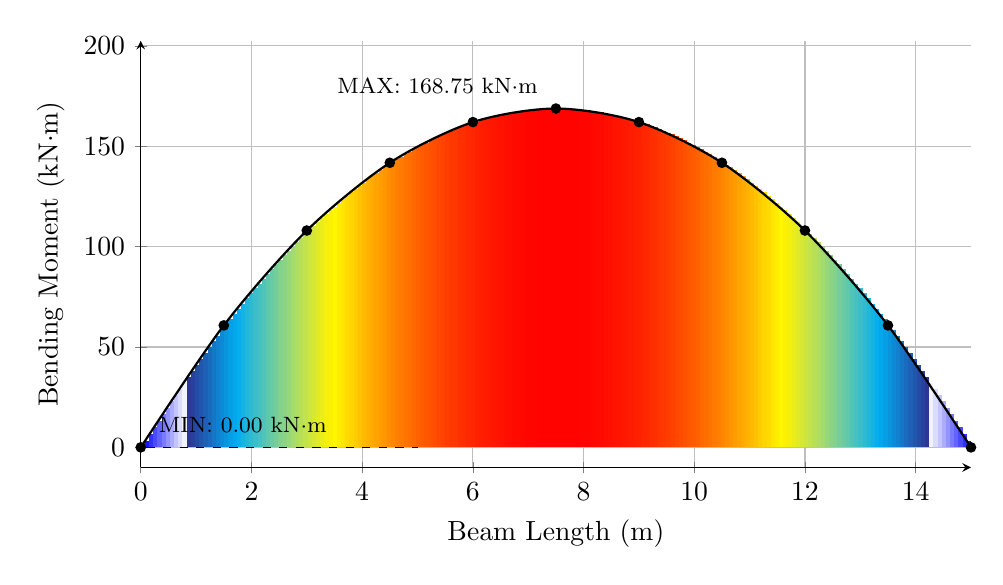
\begin{tikzpicture}
\begin{axis}[
    width=\textwidth,
    height=7cm,
    xlabel={Beam Length (m)},
    ylabel={Bending Moment (kN$\cdot$m)},
    xmin=0.000,
    xmax=15.000,
    ymin=-10.000,
    ymax=202.500,
    grid=major,
    axis lines=left
]

% Colored vertical strips for gradient effect
\fill[blue!100] (axis cs:0.0000,0) rectangle (axis cs:0.0754,0.0000);
\fill[blue!91] (axis cs:0.0754,0) rectangle (axis cs:0.1508,3.3749);
\fill[blue!81] (axis cs:0.1508,0) rectangle (axis cs:0.2261,6.7157);
\fill[blue!71] (axis cs:0.2261,0) rectangle (axis cs:0.3015,10.0225);
\fill[blue!61] (axis cs:0.3015,0) rectangle (axis cs:0.3769,13.2951);
\fill[blue!52] (axis cs:0.3769,0) rectangle (axis cs:0.4523,16.5337);
\fill[blue!42] (axis cs:0.4523,0) rectangle (axis cs:0.5276,19.7381);
\fill[blue!33] (axis cs:0.5276,0) rectangle (axis cs:0.6030,22.9085);
\fill[blue!23] (axis cs:0.6030,0) rectangle (axis cs:0.6784,26.0448);
\fill[blue!14] (axis cs:0.6784,0) rectangle (axis cs:0.7538,29.1470);
\fill[blue!5] (axis cs:0.7538,0) rectangle (axis cs:0.8291,32.2151);
\fill[cyan!4!blue] (axis cs:0.8291,0) rectangle (axis cs:0.9045,35.2491);
\fill[cyan!13!blue] (axis cs:0.9045,0) rectangle (axis cs:0.9799,38.2490);
\fill[cyan!22!blue] (axis cs:0.9799,0) rectangle (axis cs:1.0553,41.2149);
\fill[cyan!30!blue] (axis cs:1.0553,0) rectangle (axis cs:1.1307,44.1466);
\fill[cyan!39!blue] (axis cs:1.1307,0) rectangle (axis cs:1.2060,47.0443);
\fill[cyan!47!blue] (axis cs:1.2060,0) rectangle (axis cs:1.2814,49.9078);
\fill[cyan!56!blue] (axis cs:1.2814,0) rectangle (axis cs:1.3568,52.7373);
\fill[cyan!64!blue] (axis cs:1.3568,0) rectangle (axis cs:1.4322,55.5327);
\fill[cyan!72!blue] (axis cs:1.4322,0) rectangle (axis cs:1.5075,58.2940);
\fill[cyan!80!blue] (axis cs:1.5075,0) rectangle (axis cs:1.5829,61.0212);
\fill[cyan!88!blue] (axis cs:1.5829,0) rectangle (axis cs:1.6583,63.7143);
\fill[cyan!96!blue] (axis cs:1.6583,0) rectangle (axis cs:1.7337,66.3733);
\fill[yellow!2!cyan] (axis cs:1.7337,0) rectangle (axis cs:1.8090,68.9983);
\fill[yellow!8!cyan] (axis cs:1.8090,0) rectangle (axis cs:1.8844,71.5891);
\fill[yellow!13!cyan] (axis cs:1.8844,0) rectangle (axis cs:1.9598,74.1459);
\fill[yellow!18!cyan] (axis cs:1.9598,0) rectangle (axis cs:2.0352,76.6685);
\fill[yellow!23!cyan] (axis cs:2.0352,0) rectangle (axis cs:2.1106,79.1571);
\fill[yellow!27!cyan] (axis cs:2.1106,0) rectangle (axis cs:2.1859,81.6116);
\fill[yellow!32!cyan] (axis cs:2.1859,0) rectangle (axis cs:2.2613,84.0320);
\fill[yellow!37!cyan] (axis cs:2.2613,0) rectangle (axis cs:2.3367,86.4183);
\fill[yellow!41!cyan] (axis cs:2.3367,0) rectangle (axis cs:2.4121,88.7705);
\fill[yellow!46!cyan] (axis cs:2.4121,0) rectangle (axis cs:2.4874,91.0886);
\fill[yellow!51!cyan] (axis cs:2.4874,0) rectangle (axis cs:2.5628,93.3726);
\fill[yellow!55!cyan] (axis cs:2.5628,0) rectangle (axis cs:2.6382,95.6226);
\fill[yellow!59!cyan] (axis cs:2.6382,0) rectangle (axis cs:2.7136,97.8384);
\fill[yellow!64!cyan] (axis cs:2.7136,0) rectangle (axis cs:2.7889,100.0202);
\fill[yellow!68!cyan] (axis cs:2.7889,0) rectangle (axis cs:2.8643,102.1679);
\fill[yellow!72!cyan] (axis cs:2.8643,0) rectangle (axis cs:2.9397,104.2815);
\fill[yellow!76!cyan] (axis cs:2.9397,0) rectangle (axis cs:3.0151,106.3610);
\fill[yellow!80!cyan] (axis cs:3.0151,0) rectangle (axis cs:3.0905,108.4064);
\fill[yellow!84!cyan] (axis cs:3.0905,0) rectangle (axis cs:3.1658,110.4177);
\fill[yellow!88!cyan] (axis cs:3.1658,0) rectangle (axis cs:3.2412,112.3949);
\fill[yellow!92!cyan] (axis cs:3.2412,0) rectangle (axis cs:3.3166,114.3380);
\fill[yellow!96!cyan] (axis cs:3.3166,0) rectangle (axis cs:3.3920,116.2471);
\fill[yellow!99!cyan] (axis cs:3.3920,0) rectangle (axis cs:3.4673,118.1220);
\fill[red!3!yellow] (axis cs:3.4673,0) rectangle (axis cs:3.5427,119.9629);
\fill[red!7!yellow] (axis cs:3.5427,0) rectangle (axis cs:3.6181,121.7697);
\fill[red!10!yellow] (axis cs:3.6181,0) rectangle (axis cs:3.6935,123.5423);
\fill[red!14!yellow] (axis cs:3.6935,0) rectangle (axis cs:3.7688,125.2809);
\fill[red!17!yellow] (axis cs:3.7688,0) rectangle (axis cs:3.8442,126.9854);
\fill[red!20!yellow] (axis cs:3.8442,0) rectangle (axis cs:3.9196,128.6558);
\fill[red!24!yellow] (axis cs:3.9196,0) rectangle (axis cs:3.9950,130.2922);
\fill[red!27!yellow] (axis cs:3.9950,0) rectangle (axis cs:4.0704,131.8944);
\fill[red!30!yellow] (axis cs:4.0704,0) rectangle (axis cs:4.1457,133.4625);
\fill[red!33!yellow] (axis cs:4.1457,0) rectangle (axis cs:4.2211,134.9966);
\fill[red!36!yellow] (axis cs:4.2211,0) rectangle (axis cs:4.2965,136.4966);
\fill[red!39!yellow] (axis cs:4.2965,0) rectangle (axis cs:4.3719,137.9624);
\fill[red!41!yellow] (axis cs:4.3719,0) rectangle (axis cs:4.4472,139.3942);
\fill[red!44!yellow] (axis cs:4.4472,0) rectangle (axis cs:4.5226,140.7919);
\fill[red!47!yellow] (axis cs:4.5226,0) rectangle (axis cs:4.5980,142.1555);
\fill[red!50!yellow] (axis cs:4.5980,0) rectangle (axis cs:4.6734,143.4850);
\fill[red!52!yellow] (axis cs:4.6734,0) rectangle (axis cs:4.7487,144.7804);
\fill[red!55!yellow] (axis cs:4.7487,0) rectangle (axis cs:4.8241,146.0418);
\fill[red!57!yellow] (axis cs:4.8241,0) rectangle (axis cs:4.8995,147.2690);
\fill[red!59!yellow] (axis cs:4.8995,0) rectangle (axis cs:4.9749,148.4622);
\fill[red!62!yellow] (axis cs:4.9749,0) rectangle (axis cs:5.0503,149.6212);
\fill[red!64!yellow] (axis cs:5.0503,0) rectangle (axis cs:5.1256,150.7462);
\fill[red!66!yellow] (axis cs:5.1256,0) rectangle (axis cs:5.2010,151.8371);
\fill[red!68!yellow] (axis cs:5.2010,0) rectangle (axis cs:5.2764,152.8939);
\fill[red!70!yellow] (axis cs:5.2764,0) rectangle (axis cs:5.3518,153.9166);
\fill[red!72!yellow] (axis cs:5.3518,0) rectangle (axis cs:5.4271,154.9052);
\fill[red!74!yellow] (axis cs:5.4271,0) rectangle (axis cs:5.5025,155.8597);
\fill[red!76!yellow] (axis cs:5.5025,0) rectangle (axis cs:5.5779,156.7801);
\fill[red!78!yellow] (axis cs:5.5779,0) rectangle (axis cs:5.6533,157.6665);
\fill[red!79!yellow] (axis cs:5.6533,0) rectangle (axis cs:5.7286,158.5187);
\fill[red!81!yellow] (axis cs:5.7286,0) rectangle (axis cs:5.8040,159.3369);
\fill[red!82!yellow] (axis cs:5.8040,0) rectangle (axis cs:5.8794,160.1210);
\fill[red!84!yellow] (axis cs:5.8794,0) rectangle (axis cs:5.9548,160.8709);
\fill[red!85!yellow] (axis cs:5.9548,0) rectangle (axis cs:6.0302,161.5868);
\fill[red!87!yellow] (axis cs:6.0302,0) rectangle (axis cs:6.1055,162.2686);
\fill[red!88!yellow] (axis cs:6.1055,0) rectangle (axis cs:6.1809,162.9163);
\fill[red!89!yellow] (axis cs:6.1809,0) rectangle (axis cs:6.2563,163.5300);
\fill[red!90!yellow] (axis cs:6.2563,0) rectangle (axis cs:6.3317,164.1095);
\fill[red!91!yellow] (axis cs:6.3317,0) rectangle (axis cs:6.4070,164.6549);
\fill[red!92!yellow] (axis cs:6.4070,0) rectangle (axis cs:6.4824,165.1663);
\fill[red!93!yellow] (axis cs:6.4824,0) rectangle (axis cs:6.5578,165.6435);
\fill[red!94!yellow] (axis cs:6.5578,0) rectangle (axis cs:6.6332,166.0867);
\fill[red!95!yellow] (axis cs:6.6332,0) rectangle (axis cs:6.7085,166.4958);
\fill[red!96!yellow] (axis cs:6.7085,0) rectangle (axis cs:6.7839,166.8708);
\fill[red!96!yellow] (axis cs:6.7839,0) rectangle (axis cs:6.8593,167.2117);
\fill[red!97!yellow] (axis cs:6.8593,0) rectangle (axis cs:6.9347,167.5185);
\fill[red!98!yellow] (axis cs:6.9347,0) rectangle (axis cs:7.0101,167.7912);
\fill[red!98!yellow] (axis cs:7.0101,0) rectangle (axis cs:7.0854,168.0298);
\fill[red!98!yellow] (axis cs:7.0854,0) rectangle (axis cs:7.1608,168.2344);
\fill[red!99!yellow] (axis cs:7.1608,0) rectangle (axis cs:7.2362,168.4048);
\fill[red!99!yellow] (axis cs:7.2362,0) rectangle (axis cs:7.3116,168.5412);
\fill[red!99!yellow] (axis cs:7.3116,0) rectangle (axis cs:7.3869,168.6435);
\fill[red!99!yellow] (axis cs:7.3869,0) rectangle (axis cs:7.4623,168.7116);
\fill[red!99!yellow] (axis cs:7.4623,0) rectangle (axis cs:7.5377,168.7457);
\fill[red!99!yellow] (axis cs:7.5377,0) rectangle (axis cs:7.6131,168.7457);
\fill[red!99!yellow] (axis cs:7.6131,0) rectangle (axis cs:7.6884,168.7116);
\fill[red!99!yellow] (axis cs:7.6884,0) rectangle (axis cs:7.7638,168.6435);
\fill[red!99!yellow] (axis cs:7.7638,0) rectangle (axis cs:7.8392,168.5412);
\fill[red!99!yellow] (axis cs:7.8392,0) rectangle (axis cs:7.9146,168.4048);
\fill[red!98!yellow] (axis cs:7.9146,0) rectangle (axis cs:7.9899,168.2344);
\fill[red!98!yellow] (axis cs:7.9899,0) rectangle (axis cs:8.0653,168.0298);
\fill[red!98!yellow] (axis cs:8.0653,0) rectangle (axis cs:8.1407,167.7912);
\fill[red!97!yellow] (axis cs:8.1407,0) rectangle (axis cs:8.2161,167.5185);
\fill[red!96!yellow] (axis cs:8.2161,0) rectangle (axis cs:8.2915,167.2117);
\fill[red!96!yellow] (axis cs:8.2915,0) rectangle (axis cs:8.3668,166.8708);
\fill[red!95!yellow] (axis cs:8.3668,0) rectangle (axis cs:8.4422,166.4958);
\fill[red!94!yellow] (axis cs:8.4422,0) rectangle (axis cs:8.5176,166.0867);
\fill[red!93!yellow] (axis cs:8.5176,0) rectangle (axis cs:8.5930,165.6435);
\fill[red!92!yellow] (axis cs:8.5930,0) rectangle (axis cs:8.6683,165.1663);
\fill[red!91!yellow] (axis cs:8.6683,0) rectangle (axis cs:8.7437,164.6549);
\fill[red!90!yellow] (axis cs:8.7437,0) rectangle (axis cs:8.8191,164.1095);
\fill[red!89!yellow] (axis cs:8.8191,0) rectangle (axis cs:8.8945,163.5300);
\fill[red!88!yellow] (axis cs:8.8945,0) rectangle (axis cs:8.9698,162.9163);
\fill[red!87!yellow] (axis cs:8.9698,0) rectangle (axis cs:9.0452,162.2686);
\fill[red!85!yellow] (axis cs:9.0452,0) rectangle (axis cs:9.1206,161.5868);
\fill[red!84!yellow] (axis cs:9.1206,0) rectangle (axis cs:9.1960,160.8709);
\fill[red!82!yellow] (axis cs:9.1960,0) rectangle (axis cs:9.2714,160.1210);
\fill[red!81!yellow] (axis cs:9.2714,0) rectangle (axis cs:9.3467,159.3369);
\fill[red!79!yellow] (axis cs:9.3467,0) rectangle (axis cs:9.4221,158.5187);
\fill[red!78!yellow] (axis cs:9.4221,0) rectangle (axis cs:9.4975,157.6665);
\fill[red!76!yellow] (axis cs:9.4975,0) rectangle (axis cs:9.5729,156.7801);
\fill[red!74!yellow] (axis cs:9.5729,0) rectangle (axis cs:9.6482,155.8597);
\fill[red!72!yellow] (axis cs:9.6482,0) rectangle (axis cs:9.7236,154.9052);
\fill[red!70!yellow] (axis cs:9.7236,0) rectangle (axis cs:9.7990,153.9166);
\fill[red!68!yellow] (axis cs:9.7990,0) rectangle (axis cs:9.8744,152.8939);
\fill[red!66!yellow] (axis cs:9.8744,0) rectangle (axis cs:9.9497,151.8371);
\fill[red!64!yellow] (axis cs:9.9497,0) rectangle (axis cs:10.0251,150.7462);
\fill[red!62!yellow] (axis cs:10.0251,0) rectangle (axis cs:10.1005,149.6212);
\fill[red!59!yellow] (axis cs:10.1005,0) rectangle (axis cs:10.1759,148.4622);
\fill[red!57!yellow] (axis cs:10.1759,0) rectangle (axis cs:10.2513,147.2690);
\fill[red!55!yellow] (axis cs:10.2513,0) rectangle (axis cs:10.3266,146.0418);
\fill[red!52!yellow] (axis cs:10.3266,0) rectangle (axis cs:10.4020,144.7804);
\fill[red!50!yellow] (axis cs:10.4020,0) rectangle (axis cs:10.4774,143.4850);
\fill[red!47!yellow] (axis cs:10.4774,0) rectangle (axis cs:10.5528,142.1555);
\fill[red!44!yellow] (axis cs:10.5528,0) rectangle (axis cs:10.6281,140.7919);
\fill[red!41!yellow] (axis cs:10.6281,0) rectangle (axis cs:10.7035,139.3942);
\fill[red!39!yellow] (axis cs:10.7035,0) rectangle (axis cs:10.7789,137.9624);
\fill[red!36!yellow] (axis cs:10.7789,0) rectangle (axis cs:10.8543,136.4966);
\fill[red!33!yellow] (axis cs:10.8543,0) rectangle (axis cs:10.9296,134.9966);
\fill[red!30!yellow] (axis cs:10.9296,0) rectangle (axis cs:11.0050,133.4625);
\fill[red!27!yellow] (axis cs:11.0050,0) rectangle (axis cs:11.0804,131.8944);
\fill[red!24!yellow] (axis cs:11.0804,0) rectangle (axis cs:11.1558,130.2922);
\fill[red!20!yellow] (axis cs:11.1558,0) rectangle (axis cs:11.2312,128.6558);
\fill[red!17!yellow] (axis cs:11.2312,0) rectangle (axis cs:11.3065,126.9854);
\fill[red!14!yellow] (axis cs:11.3065,0) rectangle (axis cs:11.3819,125.2809);
\fill[red!10!yellow] (axis cs:11.3819,0) rectangle (axis cs:11.4573,123.5423);
\fill[red!7!yellow] (axis cs:11.4573,0) rectangle (axis cs:11.5327,121.7697);
\fill[red!3!yellow] (axis cs:11.5327,0) rectangle (axis cs:11.6080,119.9629);
\fill[yellow!99!cyan] (axis cs:11.6080,0) rectangle (axis cs:11.6834,118.1220);
\fill[yellow!96!cyan] (axis cs:11.6834,0) rectangle (axis cs:11.7588,116.2471);
\fill[yellow!92!cyan] (axis cs:11.7588,0) rectangle (axis cs:11.8342,114.3380);
\fill[yellow!88!cyan] (axis cs:11.8342,0) rectangle (axis cs:11.9095,112.3949);
\fill[yellow!84!cyan] (axis cs:11.9095,0) rectangle (axis cs:11.9849,110.4177);
\fill[yellow!80!cyan] (axis cs:11.9849,0) rectangle (axis cs:12.0603,108.4064);
\fill[yellow!76!cyan] (axis cs:12.0603,0) rectangle (axis cs:12.1357,106.3610);
\fill[yellow!72!cyan] (axis cs:12.1357,0) rectangle (axis cs:12.2111,104.2815);
\fill[yellow!68!cyan] (axis cs:12.2111,0) rectangle (axis cs:12.2864,102.1679);
\fill[yellow!64!cyan] (axis cs:12.2864,0) rectangle (axis cs:12.3618,100.0202);
\fill[yellow!59!cyan] (axis cs:12.3618,0) rectangle (axis cs:12.4372,97.8384);
\fill[yellow!55!cyan] (axis cs:12.4372,0) rectangle (axis cs:12.5126,95.6226);
\fill[yellow!51!cyan] (axis cs:12.5126,0) rectangle (axis cs:12.5879,93.3726);
\fill[yellow!46!cyan] (axis cs:12.5879,0) rectangle (axis cs:12.6633,91.0886);
\fill[yellow!41!cyan] (axis cs:12.6633,0) rectangle (axis cs:12.7387,88.7705);
\fill[yellow!37!cyan] (axis cs:12.7387,0) rectangle (axis cs:12.8141,86.4183);
\fill[yellow!32!cyan] (axis cs:12.8141,0) rectangle (axis cs:12.8894,84.0320);
\fill[yellow!27!cyan] (axis cs:12.8894,0) rectangle (axis cs:12.9648,81.6116);
\fill[yellow!23!cyan] (axis cs:12.9648,0) rectangle (axis cs:13.0402,79.1571);
\fill[yellow!18!cyan] (axis cs:13.0402,0) rectangle (axis cs:13.1156,76.6685);
\fill[yellow!13!cyan] (axis cs:13.1156,0) rectangle (axis cs:13.1910,74.1459);
\fill[yellow!8!cyan] (axis cs:13.1910,0) rectangle (axis cs:13.2663,71.5891);
\fill[yellow!2!cyan] (axis cs:13.2663,0) rectangle (axis cs:13.3417,68.9983);
\fill[cyan!96!blue] (axis cs:13.3417,0) rectangle (axis cs:13.4171,66.3733);
\fill[cyan!88!blue] (axis cs:13.4171,0) rectangle (axis cs:13.4925,63.7143);
\fill[cyan!80!blue] (axis cs:13.4925,0) rectangle (axis cs:13.5678,61.0212);
\fill[cyan!72!blue] (axis cs:13.5678,0) rectangle (axis cs:13.6432,58.2940);
\fill[cyan!64!blue] (axis cs:13.6432,0) rectangle (axis cs:13.7186,55.5327);
\fill[cyan!56!blue] (axis cs:13.7186,0) rectangle (axis cs:13.7940,52.7373);
\fill[cyan!47!blue] (axis cs:13.7940,0) rectangle (axis cs:13.8693,49.9078);
\fill[cyan!39!blue] (axis cs:13.8693,0) rectangle (axis cs:13.9447,47.0443);
\fill[cyan!30!blue] (axis cs:13.9447,0) rectangle (axis cs:14.0201,44.1466);
\fill[cyan!22!blue] (axis cs:14.0201,0) rectangle (axis cs:14.0955,41.2149);
\fill[cyan!13!blue] (axis cs:14.0955,0) rectangle (axis cs:14.1709,38.2490);
\fill[cyan!4!blue] (axis cs:14.1709,0) rectangle (axis cs:14.2462,35.2491);
\fill[blue!5] (axis cs:14.2462,0) rectangle (axis cs:14.3216,32.2151);
\fill[blue!14] (axis cs:14.3216,0) rectangle (axis cs:14.3970,29.1470);
\fill[blue!23] (axis cs:14.3970,0) rectangle (axis cs:14.4724,26.0448);
\fill[blue!33] (axis cs:14.4724,0) rectangle (axis cs:14.5477,22.9085);
\fill[blue!42] (axis cs:14.5477,0) rectangle (axis cs:14.6231,19.7381);
\fill[blue!52] (axis cs:14.6231,0) rectangle (axis cs:14.6985,16.5337);
\fill[blue!61] (axis cs:14.6985,0) rectangle (axis cs:14.7739,13.2951);
\fill[blue!71] (axis cs:14.7739,0) rectangle (axis cs:14.8492,10.0225);
\fill[blue!81] (axis cs:14.8492,0) rectangle (axis cs:14.9246,6.7157);
\fill[blue!91] (axis cs:14.9246,0) rectangle (axis cs:15.0000,3.3749);

% Zero reference line
\addplot[black, very thin, dashed] {0};

% Trajectory curve with markers
\addplot[
    black,
    thick,
    mark=*,
    mark size=1.5pt,
    smooth
] coordinates {
(0.000,0.000)
(1.500,60.750)
(3.000,108.000)
(4.500,141.750)
(6.000,162.000)
(7.500,168.750)
(9.000,162.000)
(10.500,141.750)
(12.000,108.000)
(13.500,60.750)
(15.000,0.000)
};

% MAX annotation
\node[anchor=south east, font=\footnotesize, text=black, xshift=-3pt, yshift=2pt] at (axis cs:7.500,168.750) {MAX: 168.75 kN$\cdot$m};

% MIN annotation
\node[anchor=south west, font=\footnotesize, text=black, xshift=3pt, yshift=2pt] at (axis cs:0.000,0.000) {MIN: 0.00 kN$\cdot$m};

\end{axis}
\end{tikzpicture}
\caption{Bending Moment Diagram (BMD) - Contour Visualization}
\label{fig:bmd}
\end{figure}

%
\section{Summary}%
\label{sec:Summary}%
This report has presented a complete structural analysis of a simply supported beam, %
including detailed force calculations and professional visualization of results.%
\vspace{0.3cm}%
\\%
\textbf{Key Results:}%
\begin{itemize}%
\item Maximum Shear Force: 45.00 kN%
\item Maximum Bending Moment: 168.75 kN$\cdot$m%
\item Number of Load Points: 11%
\item Beam Span: 15.00 m%
\end{itemize}%
\vspace{0.3cm}%
The analysis was performed using Python with PyLaTeX for document generation and %
pgfplots for high{-}quality vector graphics. All diagrams and tables were generated %
programmatically to ensure accuracy and reproducibility.

%
\end{document}